\documentclass[handout]{beamer}
\usepackage[utf8]{inputenc}
\usepackage[T2A]{fontenc}
\usepackage[english]{babel}
\usepackage{graphicx}
\usepackage{array}
\usetheme{Warsaw}
\usecolortheme{wolverine}

\usepackage{fontawesome5}
\usepackage{listings}
\usepackage[all]{xy}
\usepackage{changepage}

\lstset{
  language=Haskell,
  showstringspaces=false,
  columns=flexible,
  basicstyle={\ttfamily},
  numbers=none,
  numberstyle=\tiny\color{gray},
  keywordstyle=\color{blue},
  commentstyle=\color{dkgreen},
  stringstyle=\color{red},
  breaklines=true,
  breakatwhitespace=true,
  tabsize=2
}

\newtheorem{conjecture}[theorem]{$abc$ conjecture}

\def\N{\mathbb{N}}

\definecolor{darkblue}{rgb}{0,0,0.8}
\definecolor{darkgreen}{rgb}{0,0.6,0}

\def\problem{\textcolor{darkblue}{\bf Problem:} }
\def\solution{\textcolor{darkgreen}{\bf Haskell solution:} }

\title{Haskell for mathematical libraries}
\author[Andrew Lelechenko]{Andrew Lelechenko}
\institute[Barclays]{Barclays, London}
\date{Lambda Days 2020, Kraków, 13.02.2020}

\begin{document}

\begin{frame}
  \titlepage
\end{frame}

\begin{frame}{Reproducibility crisis}

\begin{itemize}[<+->]
\item \problem
  Many scientific studies are difficult or impossible to replicate or reproduce. \par~
\item
  According to 2016 poll by {\em Nature},
  70\% of 1500 participants
  failed to reproduce other scientist's experiment. \par~
\item
  {\bf Even worse:}
  50\% failed to reproduce their own experiment. \par~
\item
  Social sciences and medicine are most susceptible {\em (kinda expected)}. \par~
\item
  But are computer sciences and mathematics secure?
\end{itemize}

\end{frame}

\begin{frame}{Reproducibility crisis --- CS}

\centerline{C. Collberg, T. Proebsting, A. M. Warren,}
\centerline{{\em Repeatability and benefaction in computer systems research,} 2015.}

\bigskip

\begin{itemize}[<+->]
\item
  Collberg et al. conducted an exploration of $\sim 400$ papers
  from ACM conferences and journals.
\item
  For 32.3\% they were able to obtain the code
  and build it easily.
\item
  For 48.3\% they managed to build the code,
  but it may have required extra effort.
\item
  For 54.0\% either they managed to build the code
  or the authors stated the code would build with reasonable effort.
\end{itemize}

\end{frame}

\begin{frame}{Reproducibility crisis --- mathematics}

\begin{conjecture}
  Let $a$, $b$, $c$ be coprime positive integers such that $a+b = c$.
  Then the product of distinct prime factors of $a\cdot b\cdot c$
  is usually not much smaller than $c$:
  $$
    c > \mathrm{rad}(abc)^{1+\varepsilon}.
  $$
\end{conjecture}

\begin{itemize}[<+->]
\item
  In 2012 Shinichi Mochizuki outlined a proof on 500 pages.
\item
  In 2015--2016 several workshops
  tried to grasp his ideas.
\item
  In 2017 Go Yamashita published 300 pages of explanations.
\item
  In 2018 Peter Scholze and Jakob Stix identified a gap.
\item
  Mochizuki claimed that they misunderstood vital aspects
  of the theory and made invalid simplifications.
\end{itemize}

\end{frame}


\begin{frame}{Concrete math}

\begin{quotation}
If I can give an abstract proof of something,
I'm reasonably happy. But if I can get a concrete,
computational proof and actually produce numbers
I'm much happier. I'm rather an addict of doing things
on the computer.

\hfill John Milnor
\end{quotation}

\bigskip

\pause

\begin{quotation}
As a computational and experimental pure mathematician
my main goal is: {\sf insight}. \ldots
This is leading us towards an {\sf Experimental M{\bf a}thodology}
as a philosophy and in practice.

\hfill Jonathan M. Borwein,

\hfill \AE sthetics for the working mathematician, 2001.
\end{quotation}

\end{frame}

\title{Haskell for the working mathematician}

\begin{frame}
  \titlepage
\end{frame}


\begin{frame}{Boolean blindness}

{\bf Antipattern:}
use {\tt Bool} to represent any type with two values:

\medskip

\centerline{\tt data Bool = True | False}

\bigskip

\pause

{\bf Example:}

\centerline{\tt filter :: (a -> Bool) -> [a] -> [a]}

\medskip

Does {\tt True} mean to keep or to discard here?

\bigskip

\pause

{\bf Pattern:} use a domain-specific type.

\medskip

\centerline{\tt data Action = Keep | Discard}

\end{frame}

\begin{frame}{Int blindness and nominal typing}

{\bf Antipattern:}
\par
{\tt substring :: Int -> Int -> String -> String}

\medskip

Is the second {\tt Int} an offset or a count?

\bigskip

\pause

{\bf Pattern:} use new types to wrap {\tt Int}s
and name them differently.

\medskip

{\tt newtype Offset = Offset Int } \par
{\tt newtype Count  = Count  Int } \par
{\tt substring :: Offset -> Count -> String -> String }

\bigskip

\pause

{\bf Question:} would named arguments help?

\end{frame}

\begin{frame}{Int blindness and nominal typing --- 2}

{\bf Answer:} not really. Named arguments do not prohibit invalid operations:

\pause

\begin{itemize}
\item {\tt Count  + Count  = Count }\pause
\item {\tt Offset + Count  = Offset }\pause
\item {\tt Count  + Offset = ? }\pause
\item {\tt Offset + Offset = ?}\pause
\end{itemize}

\bigskip

{\bf Real world example:}

\medskip

{\tt montgomeryFactorisation :: } \par
{\tt  ~ Integer -> Word -> Word -> Integer -> Maybe Integer }

\end{frame}

\title{LAPACK User Guide, 3rd ed., 1999}
\author[]{}

\begin{frame}{Too many types!}
\begin{figure}[H]
\centering
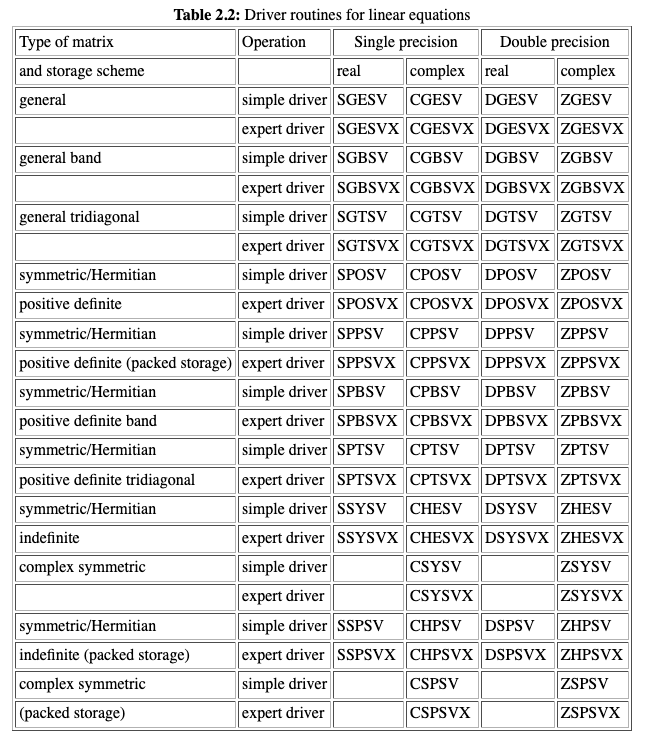
\includegraphics[width=0.9\textwidth]{lapack.png}
\end{figure}
\end{frame}

\title{Haskell for mathematical libraries}
\author[Andrew Lelechenko]{Andrew Lelechenko}

\begin{frame}{A taste of abstract algebra}

\begin{itemize}[<+->]
\item A set with an associative operation $\cdot$ such that $a\cdot(b\cdot c) = (a\cdot b)\cdot c$
  is called a {\em semigroup}.
\item If there is a neutral element, it is a {\em monoid}.
\item And if the operation is invertible, it is a {\em group}.
\item And if it commutes (so that $a \cdot b = b \cdot a$), it is an {\em abelian group}.

    \bigskip

\item A set with two sufficiently good operations may appear to be
  a~{\em semiring}, a {\em ring}, a {\em rng} or {\em rig}.
\item And if these operations are extraordinary good and fit for each other,
  it may even play out
  to be a {\em domain} or a {\em field}.
\end{itemize}

\end{frame}

\begin{frame}{Type classes for the rescue}

\begin{columns}[onlytextwidth,T]
  \begin{column}{.45\linewidth}

\begin{itemize}[<+->]
\item
  \solution
  Type classes for ad-hoc polymorphism.
\item
  \problem
  Vanilla numeric classes
  are notoriously
  unfit for mathematics.
\item
  \solution
  Use {\tt algebra} package, which offers
  a hierarchy of 100+ numeric classes,
  carefully reflecting algebraic structures.

\item
  \textcolor{darkblue}{\bf Any problems?}

\end{itemize}

  \end{column}
  \begin{column}{.5\linewidth}
    \vspace{-2ex}

    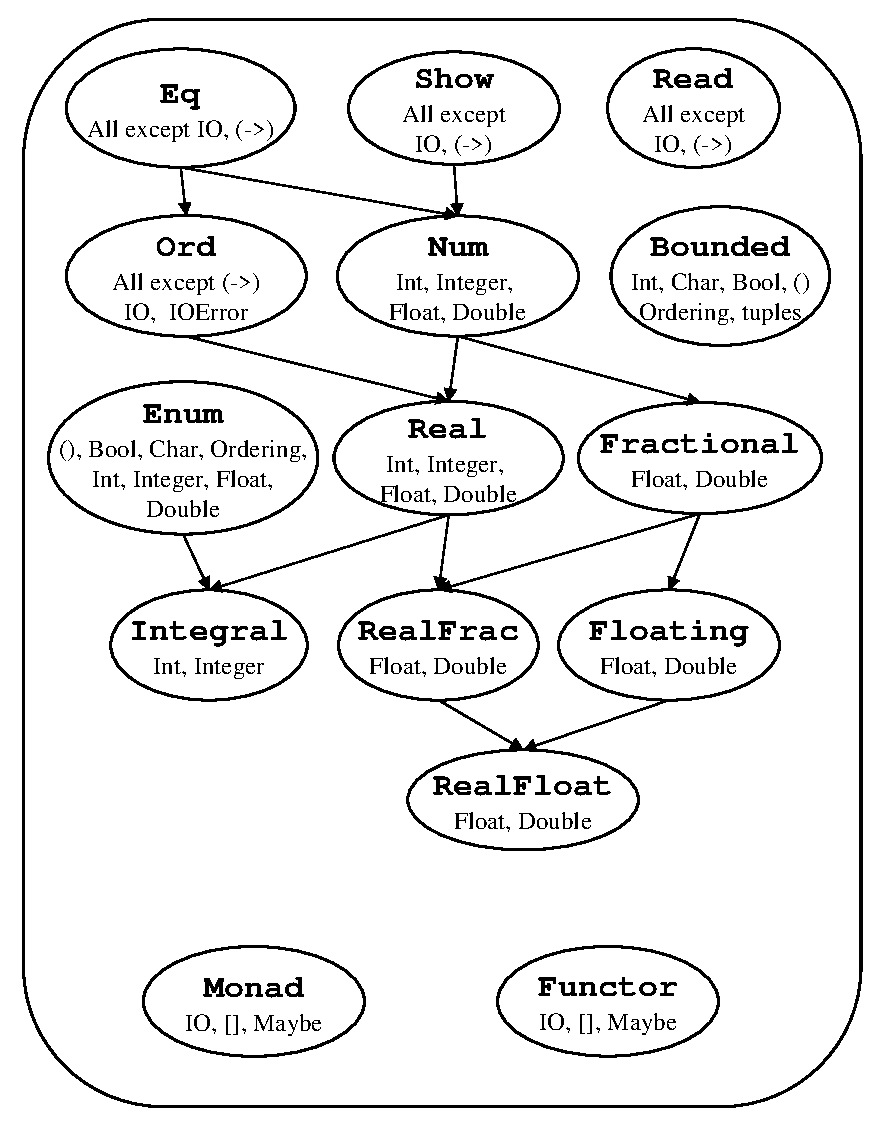
\includegraphics[width=1.05\textwidth]{classes.eps}

    \vspace{-3.5ex}

    \begin{flushright}
      {\tiny
      The Haskell 2010 Report, S.~Marlow (ed.), 2010
      }
    \end{flushright}
  \end{column}
\end{columns}

\end{frame}

\begin{frame}{Linear algebra}

\problem
The determinant is defined only for square matrices.
Multiplication is defined only if the width of the first argument
matches the height of the second one.

\medskip

{\tt det :: Matrix -> Maybe Double} \par
{\tt mul :: Matrix -> Matrix -> Maybe Matrix}

\bigskip

\pause

\solution
Parametrize matrices by phantom type-level numbers.
E. g., {\tt Matrix 3 3}, {\tt Matrix 2 4}.

\medskip

{\tt det :: Matrix n n -> Double} \par
{\tt mul :: Matrix k l -> Matrix l m -> Matrix k m}

\end{frame}

\begin{frame}{Modular arithmetic in cryptography}

\problem
In modular arithmetic all values
are reduced by modulo. Values with different moduli
are incompatible.

\medskip

{\tt newtype Mod = Mod Int Int } \par
~\par
{\tt (+) :: Mod -> Mod -> Maybe Mod } \par
{\tt Mod n mod + Mod n' mod'  } \par
{\tt ~ | mod == mod' = Just (Mod ((n + n') `rem` mod)) mod } \par
{\tt ~ | otherwise ~ = Nothing}

\medskip
{\tt Mod 4 7 + Mod 5 7 = ?}

\bigskip

\pause

\solution
Parametrize modular values by phantom type-level numbers.

\medskip

{\tt data Mod (mod :: Nat) = Mod Int } \par
{\tt (+) :: Mod m -> Mod m -> Mod m } \par

\end{frame}

\begin{frame}{Singleton values}

\begin{definition}
An integer $r$ is a square root of $n$ modulo $m$ when $r^2 \equiv n \pmod m$.
\end{definition}

{\tt sqrtMod :: Mod m -> Maybe (Mod m) } \par
{\tt sqrtMod (Mod 4 :: Mod 5) = Just (3 :: Mod 5) }

\medskip

\pause

\problem
The algorithm requires prime factorisation of $m$,
which is expensive to compute each time we need {\tt sqrtMod}:

\medskip

{\tt factorise :: Int -> [(Int, Int)] } \par
{\tt factorise 60 = [(2, 2), (3, 1), (5, 1)] } \par

\bigskip

\pause

Never forget to take a leverage of nominal types!

{\tt factorise :: Int -> [(Prime, Power)] } \par

\end{frame}


\begin{frame}{Singleton values --- 2}

{\tt sqrtMod :: Mod m -> Maybe (Mod m) }

\medskip

{\tt sqrtMod :: [(Prime, Power)] -> Mod m -> Maybe (Mod m)}

\medskip

\pause

\solution
Use singleton types, which establish a bijection between a type-level index
and its property, represented at the term level. Define

\medskip

{\tt newtype SFactors m = SFactors [(Prime, Power)] }

\medskip

and ensure by smart constructors that it has a single inhabitant.

\medskip

{\tt sqrtMod :: SFactors m -> Mod m -> Maybe (Mod m)}

\end{frame}

\begin{frame}{Lazy factorization}

\begin{itemize}[<+->]

\item Prime factorisation is very expensive:

  \smallskip

{\tt factorise :: Int -> [(Prime, Power)] } \par
{\tt factorise 60 = [(2, 2), (3, 1), (5, 1)] } \par

\item
\problem
What if further computations depend only on the first factor?
Should we expose more helpers?

  \smallskip

{\tt firstFactor :: Int -> (Prime, Power, Int)}

\item
\solution
  In a lazy language an output list is computed only on demand.
  If we consume only its head, other elements are not computed at all.
  This helps to keep API neat and concise.

  \smallskip

  {\tt firstFactor = head . factorise }

\end{itemize}

\end{frame}


\begin{frame}{Recurrent sequences}

\problem Here are Fibonacci numbers:

\vspace{-3ex}

  \begin{align*}
  F_0 &= 0  \\
  F_1 &= 1  \\
  F_n &= F_{n-1} + F_{n-2}
  \end{align*}

\pause

\textcolor{darkgreen}{\bf Naive solution:}

\medskip

  {\tt fib :: Int -> Int } \par
  {\tt fib n = if n < 2 then n else fib (n-1) + fib (n-2) }

\medskip

\pause

\solution Use a lazy list as a cache:

\medskip

  {\tt fibs :: [Int]} \par
  {\tt fibs = 0 : 1 : zipWith (+) fibs (tail fibs) }

\end{frame}


\begin{frame}{Riemann zeta function}

\problem
% Here is the Riemann zeta function $\zeta(n)$ from
{\em Computational strategies for the Riemann zeta function}
by Borwein et~al., 2000:

\begin{multline*}
- \frac{(1-2^{-2m-1}) 2 \textcolor{red}{\zeta(2m+1)}}{ (\pi i)^{2m}}
=
\sum_{k=1}^{m-1} \frac{(1-4^{-k}) \textcolor{red}{\zeta(2k+1)}}{(\pi i)^{2k} (2m-2k)! }
+ \\ +
\frac{1}{(2m)!} \left\{
  \log 2 - \frac{1}{2m} + \sum_{n=1}^\infty \frac{\zeta(2n)}{4^n (n+m)}.
\right\}
\end{multline*}

\pause

\solution
There is a generic approach to memoize recurrent sequences,
using fix-point combinator and higher-order functions.
Moreover, one can split such computation into
an actual computation and memoization layer,
which can be composed independently.

\end{frame}

\begin{frame}{Fix-point combinator}

This is a fix-point combinator:

\medskip

{\tt fix :: (a -> a) -> a} \par
{\tt fix f = f (fix f) }

\medskip

\pause

These are our na\"{\i}ve Fibonacci numbers:

\medskip

  {\tt fib :: Int -> Int } \par
  {\tt fib n = if n < 2 then n else fib (n-1) + fib (n-2) }

\medskip

\pause

These are Fibonacci numbers with recursion factored out:

\medskip

{\tt fibF :: (Int -> Int) -> Int -> Int} \par
{\tt fibF f n = if n < 2 then n else f (n-1) + f (n-2)}

\end{frame}


\begin{frame}{Conclusion}

\begin{itemize}
\item
  \problem mathematical objects are pure, immutable and lazy. \pause
\item
  \textcolor{darkgreen}{\bf Solution:}
  Haskell is pure, immutable and lazy. \pause
\end{itemize}

% concise API because of type classes
% precise types
% laziness

\bigskip
\bigskip
\bigskip
\bigskip

\centerline{\Huge\bf Thank you!}

\bigskip

{\tt https://github.com/Bodigrim/\{arithmoi,chimera,mod,poly\}}

\end{frame}

\end{document}
